% !TEX root = ../main.tex

\section{Introduction}

This report provides an overview of the Entrained Flow Reactor (EFR) at NREL. The reactor operates at fast pyrolysis conditions to thermochemically convert biomass into gaseous products. The EFR is part of the Thermochemical Process Development Unit (TCPDU) at NREL which was originally designed for biomass gasification where the EFR was used as a thermal cracker. An overview of the TCPDU system is shown in Figure \ref{fig:tcpdu-system}.

\begin{figure}[H]
    \centering
    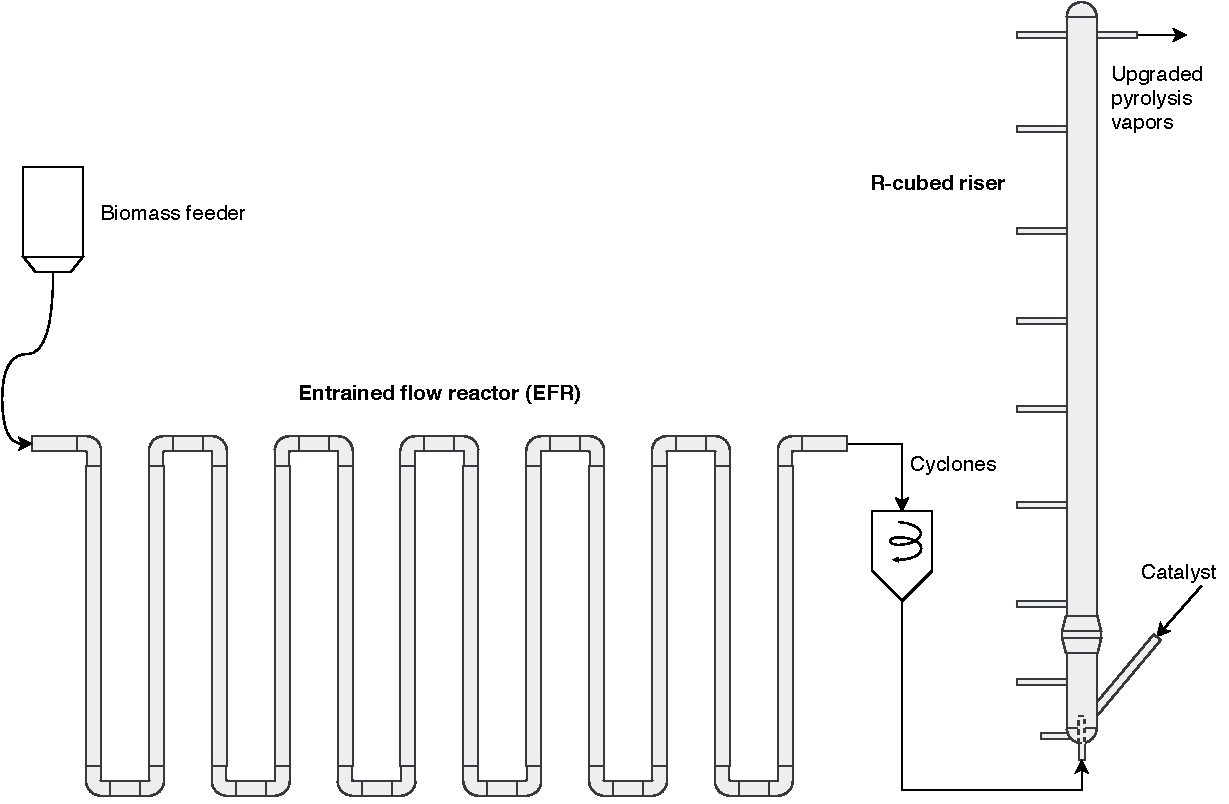
\includegraphics[width=\textwidth]{figures/tcpdu-system.pdf}
    \caption{Overview of the main components of the NREL TCPDU system. Fast pyrolysis of biomass occurs in the entrained flow reactor. Catalytic vapor phase upgrading occurs in the R-cubed riser reactor.}
    \label{fig:tcpdu-system}
\end{figure}
